\documentclass{beamer}

% Solarized Theme
\usecolortheme[light, accent=orange]{solarized}
\beamertemplatenavigationsymbolsempty

% Packages
\usepackage[T1]{fontenc}
\usepackage[utf8]{inputenc}
\usepackage[english]{babel}

\usepackage{amsmath}
\usepackage{tikz}
\usepackage{tikzsymbols}
\usetikzlibrary{positioning, math, automata}
\usepackage{blkarray}
\usepackage{graphicx}
\usepackage{multicol}
\usepackage{fontawesome}

\title{A 3-player game theoretic model of a choice between two queueing systems with strategic managerial decision making}
\author{\textbf{Michalis Panayides}}
\date{}

\begin{document}
    \frame{
        \titlepage
        \centering
        \vspace{-2cm}
        \textbf{EURO 2021 Athens}
    }
    \setbeamertemplate{frametitle}[default][center]
    
    \begin{frame}
    \frametitle{Queues}
    \centering

    
\includegraphics[scale=0.3]{Bin/supermarket-queue.jpg}
    
\includegraphics[scale=0.3]{Bin/supermarket-queue.jpg}
    
\includegraphics[scale=0.3]{Bin/supermarket-queue.jpg}
\end{frame}


\begin{frame}
    \frametitle{Queues}
    \centering

    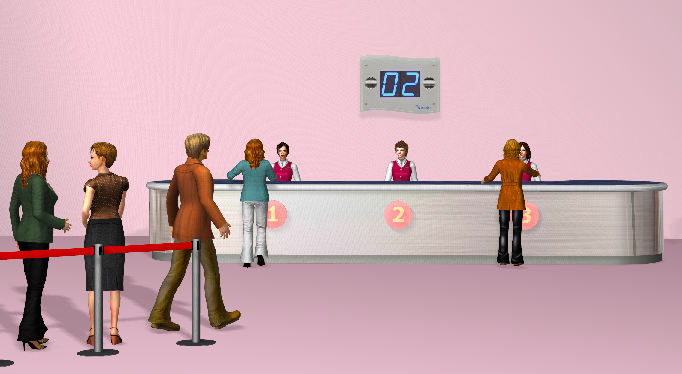
\includegraphics[scale=0.55]{Bin/bank-queue.png}
\end{frame}


\begin{frame}
    \frametitle{Queues}
    \centering
    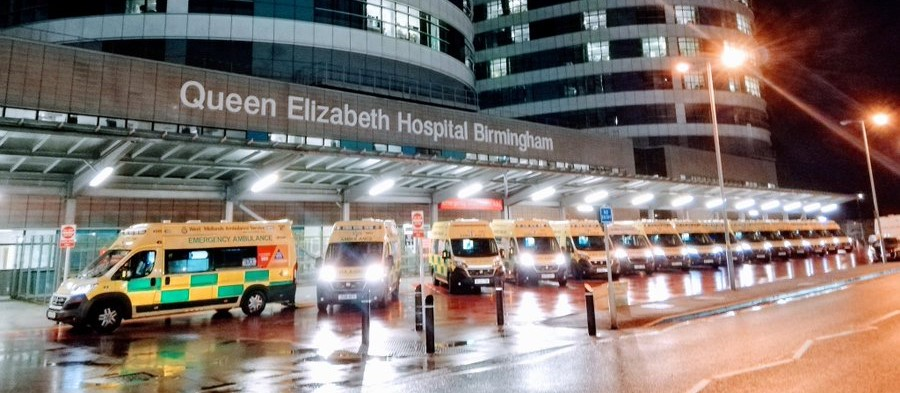
\includegraphics[scale=0.45]{Bin/ambulance_queue.jpg}
\end{frame}
    \begin{frame}
    \frametitle{Queues}
    \centering

    
\includegraphics[scale=0.3]{Bin/supermarket-queue.jpg}
    
\includegraphics[scale=0.3]{Bin/supermarket-queue.jpg}
    
\includegraphics[scale=0.3]{Bin/supermarket-queue.jpg}
\end{frame}


\begin{frame}
    \frametitle{Queues}
    \centering

    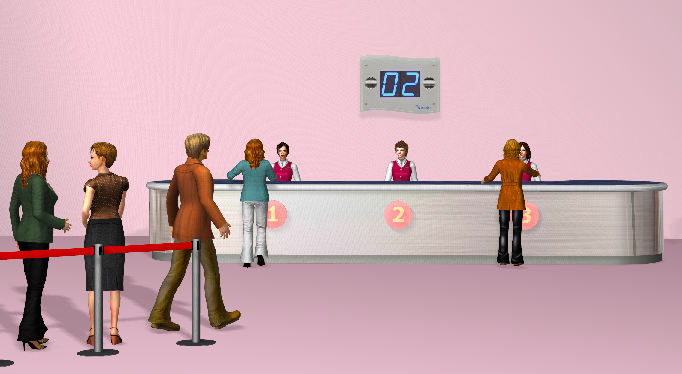
\includegraphics[scale=0.55]{Bin/bank-queue.png}
\end{frame}


\begin{frame}
    \frametitle{Queues}
    \centering
    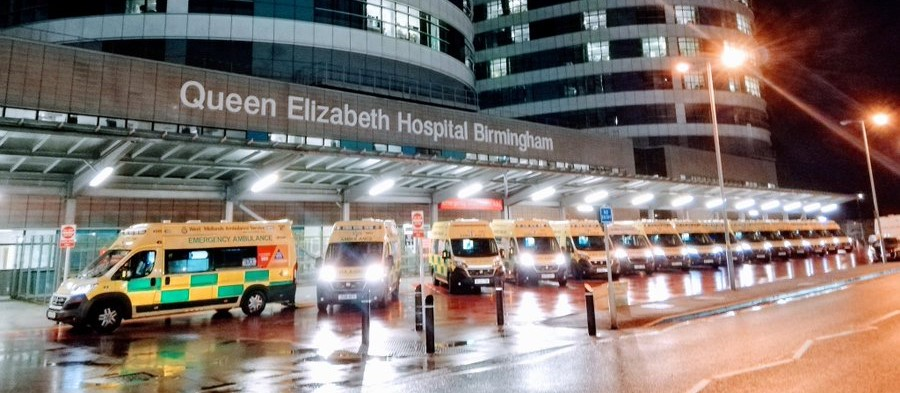
\includegraphics[scale=0.45]{Bin/ambulance_queue.jpg}
\end{frame}
    \begin{frame}
    \frametitle{Queues}
    \centering

    
\includegraphics[scale=0.3]{Bin/supermarket-queue.jpg}
    
\includegraphics[scale=0.3]{Bin/supermarket-queue.jpg}
    
\includegraphics[scale=0.3]{Bin/supermarket-queue.jpg}
\end{frame}


\begin{frame}
    \frametitle{Queues}
    \centering

    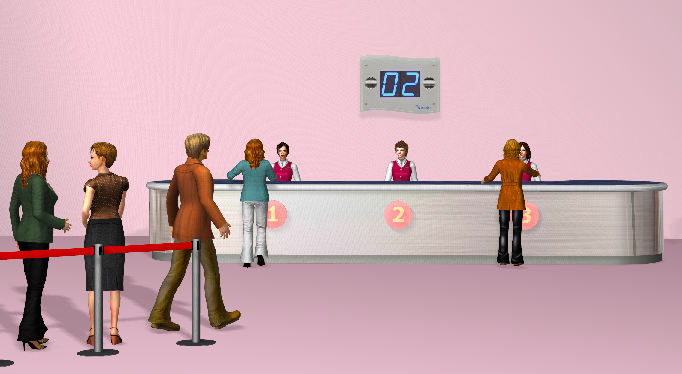
\includegraphics[scale=0.55]{Bin/bank-queue.png}
\end{frame}


\begin{frame}
    \frametitle{Queues}
    \centering
    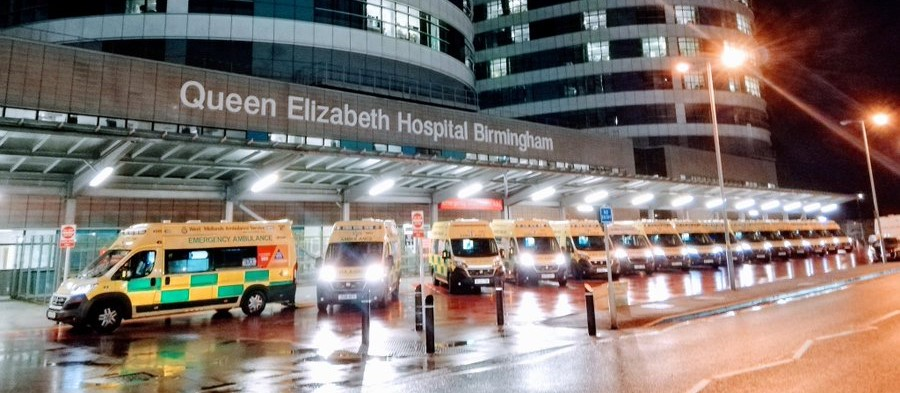
\includegraphics[scale=0.45]{Bin/ambulance_queue.jpg}
\end{frame}
    \begin{frame}
    \frametitle{Queues}
    \centering

    
\includegraphics[scale=0.3]{Bin/supermarket-queue.jpg}
    
\includegraphics[scale=0.3]{Bin/supermarket-queue.jpg}
    
\includegraphics[scale=0.3]{Bin/supermarket-queue.jpg}
\end{frame}


\begin{frame}
    \frametitle{Queues}
    \centering

    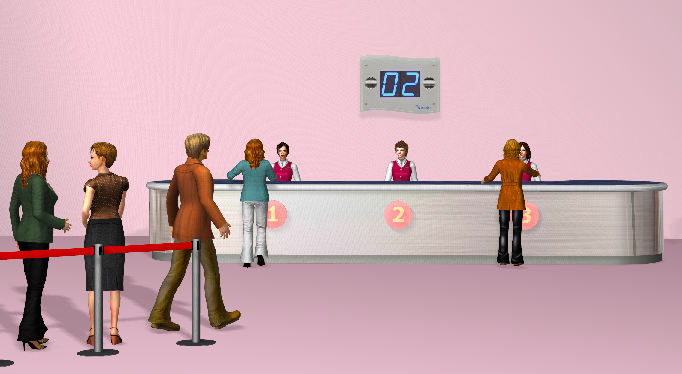
\includegraphics[scale=0.55]{Bin/bank-queue.png}
\end{frame}


\begin{frame}
    \frametitle{Queues}
    \centering
    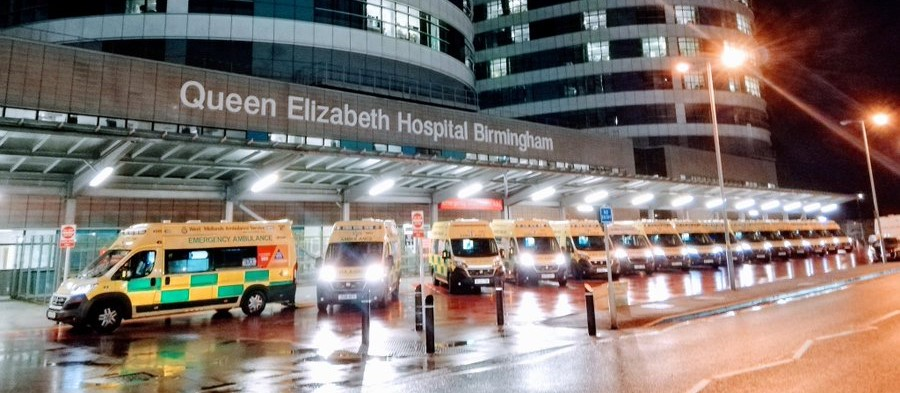
\includegraphics[scale=0.45]{Bin/ambulance_queue.jpg}
\end{frame}
    \begin{frame}
    \frametitle{Queues}
    \centering

    
\includegraphics[scale=0.3]{Bin/supermarket-queue.jpg}
    
\includegraphics[scale=0.3]{Bin/supermarket-queue.jpg}
    
\includegraphics[scale=0.3]{Bin/supermarket-queue.jpg}
\end{frame}


\begin{frame}
    \frametitle{Queues}
    \centering

    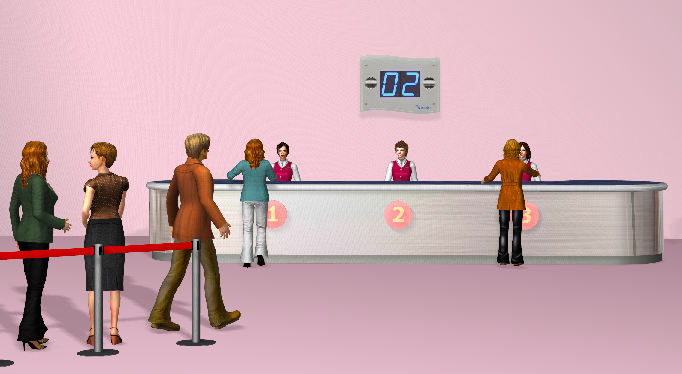
\includegraphics[scale=0.55]{Bin/bank-queue.png}
\end{frame}


\begin{frame}
    \frametitle{Queues}
    \centering
    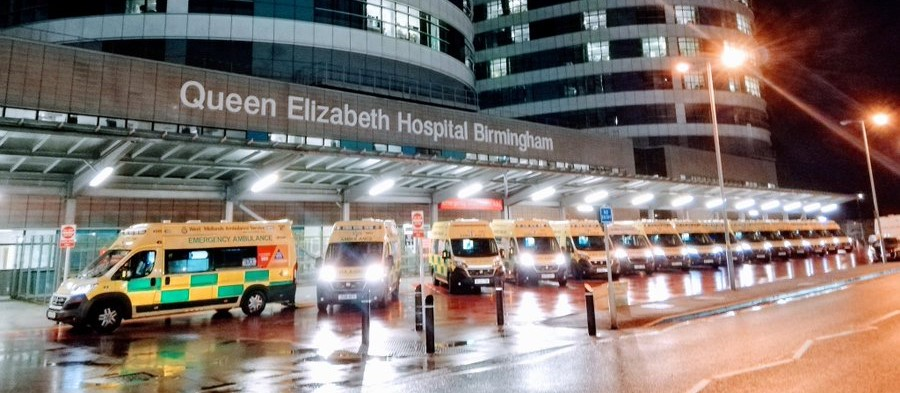
\includegraphics[scale=0.45]{Bin/ambulance_queue.jpg}
\end{frame}
    \begin{frame}
    \frametitle{Queues}
    \centering

    
\includegraphics[scale=0.3]{Bin/supermarket-queue.jpg}
    
\includegraphics[scale=0.3]{Bin/supermarket-queue.jpg}
    
\includegraphics[scale=0.3]{Bin/supermarket-queue.jpg}
\end{frame}


\begin{frame}
    \frametitle{Queues}
    \centering

    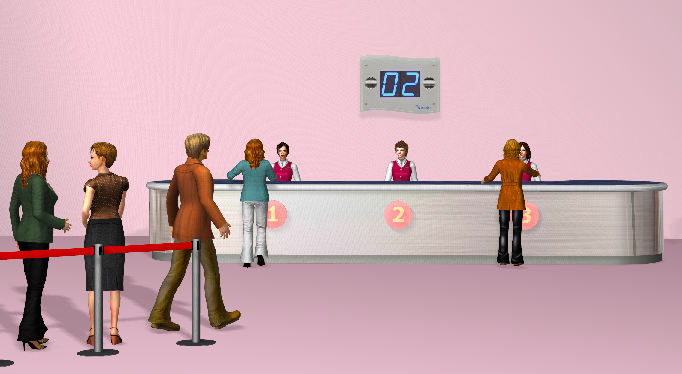
\includegraphics[scale=0.55]{Bin/bank-queue.png}
\end{frame}


\begin{frame}
    \frametitle{Queues}
    \centering
    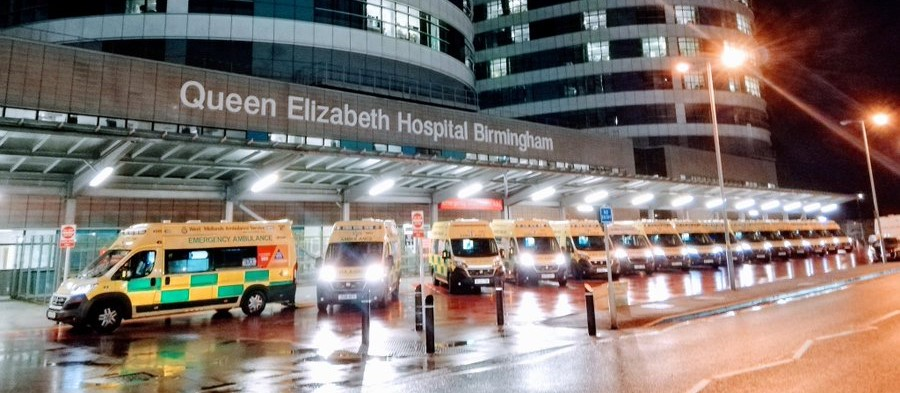
\includegraphics[scale=0.45]{Bin/ambulance_queue.jpg}
\end{frame}
    \begin{frame}
    \frametitle{Queues}
    \centering

    
\includegraphics[scale=0.3]{Bin/supermarket-queue.jpg}
    
\includegraphics[scale=0.3]{Bin/supermarket-queue.jpg}
    
\includegraphics[scale=0.3]{Bin/supermarket-queue.jpg}
\end{frame}


\begin{frame}
    \frametitle{Queues}
    \centering

    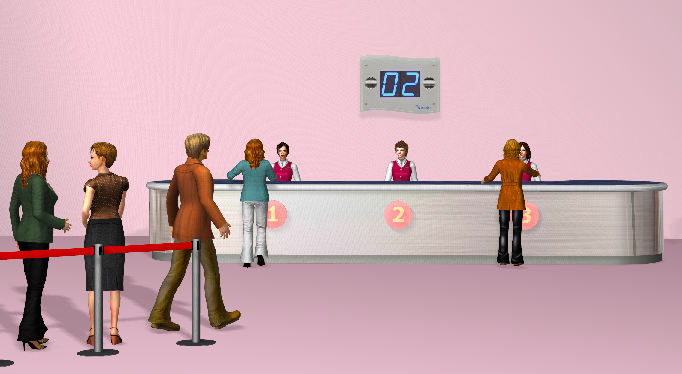
\includegraphics[scale=0.55]{Bin/bank-queue.png}
\end{frame}


\begin{frame}
    \frametitle{Queues}
    \centering
    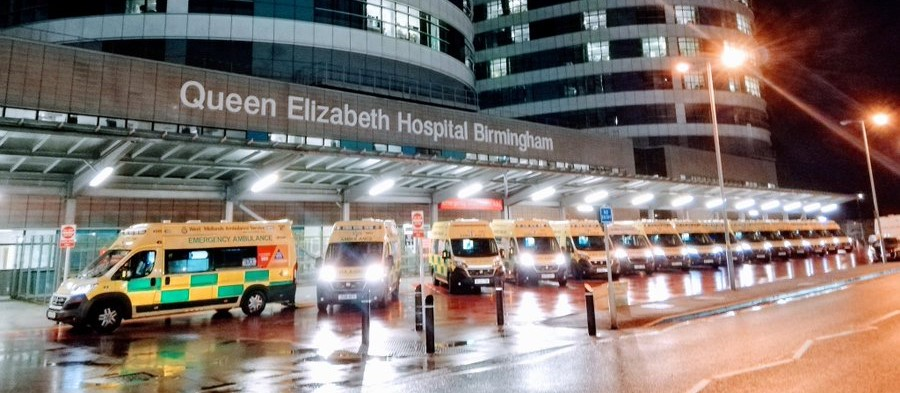
\includegraphics[scale=0.45]{Bin/ambulance_queue.jpg}
\end{frame}
    \begin{frame}
    \frametitle{Queues}
    \centering

    
\includegraphics[scale=0.3]{Bin/supermarket-queue.jpg}
    
\includegraphics[scale=0.3]{Bin/supermarket-queue.jpg}
    
\includegraphics[scale=0.3]{Bin/supermarket-queue.jpg}
\end{frame}


\begin{frame}
    \frametitle{Queues}
    \centering

    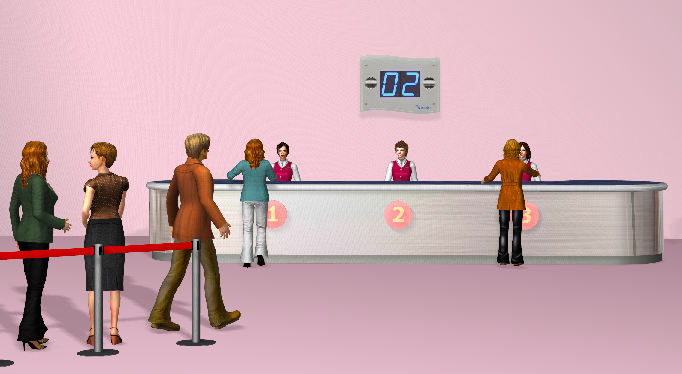
\includegraphics[scale=0.55]{Bin/bank-queue.png}
\end{frame}


\begin{frame}
    \frametitle{Queues}
    \centering
    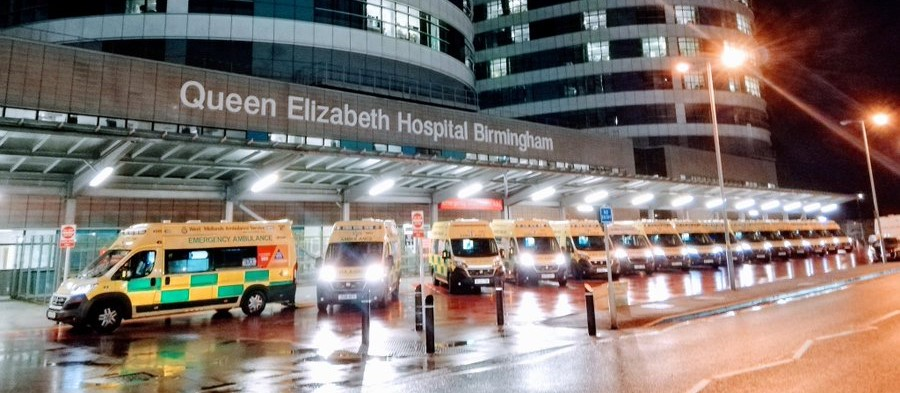
\includegraphics[scale=0.45]{Bin/ambulance_queue.jpg}
\end{frame}
    \begin{frame}
    \frametitle{Queues}
    \centering

    
\includegraphics[scale=0.3]{Bin/supermarket-queue.jpg}
    
\includegraphics[scale=0.3]{Bin/supermarket-queue.jpg}
    
\includegraphics[scale=0.3]{Bin/supermarket-queue.jpg}
\end{frame}


\begin{frame}
    \frametitle{Queues}
    \centering

    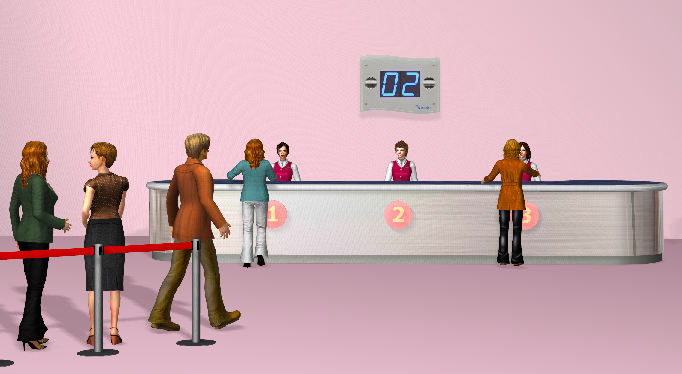
\includegraphics[scale=0.55]{Bin/bank-queue.png}
\end{frame}


\begin{frame}
    \frametitle{Queues}
    \centering
    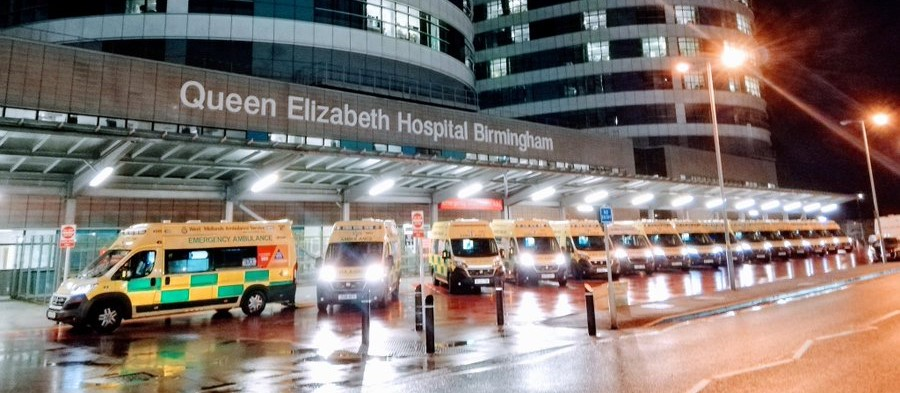
\includegraphics[scale=0.45]{Bin/ambulance_queue.jpg}
\end{frame}
    \begin{frame}
    \frametitle{Queues}
    \centering

    
\includegraphics[scale=0.3]{Bin/supermarket-queue.jpg}
    
\includegraphics[scale=0.3]{Bin/supermarket-queue.jpg}
    
\includegraphics[scale=0.3]{Bin/supermarket-queue.jpg}
\end{frame}


\begin{frame}
    \frametitle{Queues}
    \centering

    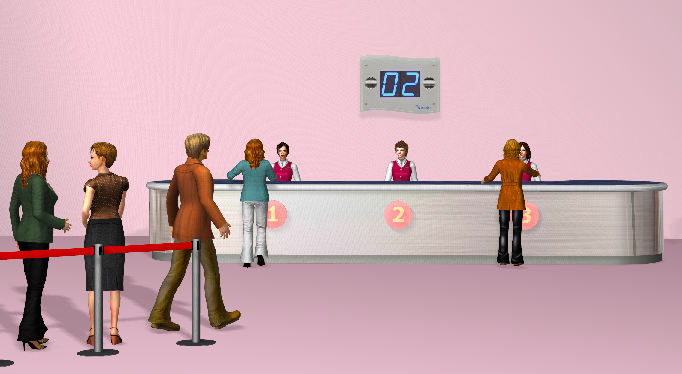
\includegraphics[scale=0.55]{Bin/bank-queue.png}
\end{frame}


\begin{frame}
    \frametitle{Queues}
    \centering
    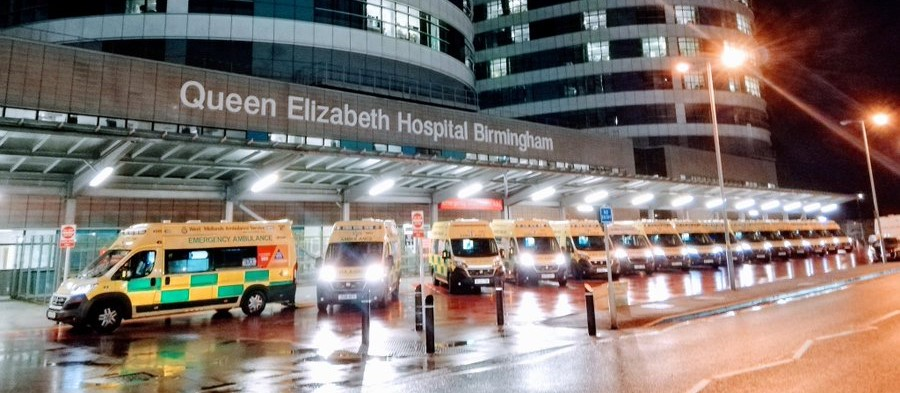
\includegraphics[scale=0.45]{Bin/ambulance_queue.jpg}
\end{frame}

\end{document}